% defer/rcuintro.tex
% mainfile: ../perfbook.tex
% SPDX-License-Identifier: CC-BY-SA-3.0

\subsection{Introduction to RCU}
\label{sec:defer:Introduction to RCU}

앞의 섹션들에서 이야기된 접근법들은 좋은 확장성을 제공하지만 분명 Pre-BSD
라우팅 테이블에 이상적이진 않은 성능을 제공했습니다.
따라서, ``오직 너무 멀리 가본 사람만이 자기가 얼마나 멀리 갈 수 있는지 안다''
정신에 입각해,\footnote{
	T.~S.~Eliot 에게 사과드립니다.}
동시의 업데이트의 존재에도 불구하고 동시의 읽기 쓰레드들이 싱글 쓰레드
탐색에서와 동일한 어셈블리 언어 인스트럭션들을 수행하는 알고리즘을 통해 더 멀리
가보겠습니다.
물론, 이 칭찬할 만한 목표는 심각한 구현 가능성 질문을 불러일으킬 수
있겠습니다만, 시도도 하지 않으면 성공할 수도 없습니다!

\iffalse

The approaches discussed in the preceding sections have provided
good scalability but decidedly non-ideal performance for the
Pre-BSD routing table.
Therefore, in the spirit of ``only those who have gone too far
know how far you can go'',\footnote{
	With apologies to T.~S.~Eliot.}
we will go all the way, looking into algorithms in which concurrent
readers execute the same sequence of assembly language instructions as
would a single-threaded lookup, despite the presence of concurrent
updates.
Of course, this laudable goal might raise serious implementability
questions, but we cannot possibly succeed if we don't even try!

\fi

\subsubsection{Minimal Insertion and Deletion}
\label{sec:defer:Minimal Insertion and Deletion}

\begin{figure}[tb]
\centering
\resizebox{3in}{!}{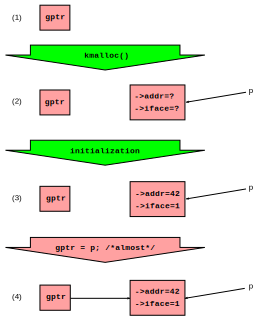
\includegraphics{defer/RCUListInsertClassic}}
\caption{Insertion With Concurrent Readers}
\label{fig:defer:Insertion With Concurrent Readers}
\end{figure}

구현이 가능하긴 한지에 대한 걱정을 최소화 하기 위해, \co{NULL} 이거나 하나의
구조체로의 참조일 하나의 글로벌 포인터로 존재하는 최소한의 데이터 구조에 집중해
봅니다.
이 데이터 구조는 최소한의 것이긴 하지만, 제품 단계에서 상당히 많이 사용되는
것이기도 합니다~\cite{GeoffRomer2018C++DeferredReclamationP0561R4}.
삽입을 위한 고전적 방법이
Figure~\ref{fig:defer:Insertion With Concurrent Readers}
에 보여져 있는데, 위에서 아래로 시간이 흐름에 따라 달라지는 네개의 상태를
보입니다.
첫번째 열은 최초의 상태를 보이는데, \co{gptr} 이 \co{NULL} 입니다.
두번째 열에서, 우리는 물음표로 보여지듯 초기화 되지 않은 이 구조체를
할당합니다.
세번째 열에서, 우린 이 구조체를 초기화 합니다.
마지막으로, 네번째 열에서 우린 \co{gptr} 을 이 새로 할당되고 초기화 된 원소를
참조하도록 업데이트 합니다.

\iffalse

To minimize implementability concerns, we focus on a minimal
data structure, which consists of a single global pointer that is either
\co{NULL} or references a single structure.
Minimal though it might be, this data structure is heavily used in
production~\cite{GeoffRomer2018C++DeferredReclamationP0561R4}.
A classic approach for insertion is shown in
Figure~\ref{fig:defer:Insertion With Concurrent Readers},
which shows four states with time advancing from top to bottom.
The first row shows the initial state, with \co{gptr} equal to \co{NULL}.
In the second row, we have allocated a structure which is uninitialized,
as indicated by the question marks.
In the third row, we have initialized the structure.
Finally, in the fourth and final row, we have updated \co{gptr} to
reference the newly allocated and initialized element.

\fi

우린 이 \co{gptr} 로의 값 할당이 간단한 C-언어의 할당문을 사용할 수 있길 바랄
겁니다.
불행히도,
Section~\ref{sec:toolsoftrade:Shared-Variable Shenanigans}
이 이 바람을 가로막습니다.
따라서, 업데이트 쓰레드는 간단한 C-언어 할당문 대신 이 그림에 보여진 것처럼
\co{smp_store_release()} 또는 뒤에서 보이겠지만 \co{rcu_assign_pointer()} 를
사용해야 합니다.

비슷하게, 어떤 사람들은 읽기 쓰레드가 \co{gptr} 의 값을 얻어오기 위해 하나의
C-언어 할당문을 사용할 수 있기를, 그리고 과거의 값인 \co{NULL} 이나 새로이
설치된 포인터를 읽어와 어떤 경우든 유효한 값을 읽올 것이 보장되기를 바랄
겁니다.
불행히도,
Section~\ref{sec:toolsoftrade:Shared-Variable Shenanigans}
은 이 바람 역시 가로막습니다.
이 보장을 얻기 위해선, 읽기 쓰레드는 그 대신 \co{READ_ONCE()}, 또는, 뒤에서
보이겠지만 \co{rcu_dereference()} 를 사용해야 합니다.
하지만, 대부분의 현대 컴퓨터 시스템에서, 이 읽기 쪽 기능들은 싱글 쓰레드 기반
코드에서 일반적으로 사용될 것과 동일한 하나의 로드 인스트럭션으로 구현될 수
있습니다.

\iffalse

We might hope that this assignment to \co{gptr} could use a simple
C-language assignment statement.
Unfortunately,
Section~\ref{sec:toolsoftrade:Shared-Variable Shenanigans}
dashes these hopes.
Therefore, the updater cannot use a simple C-language assignment, but
must instead use \co{smp_store_release()} as shown in the figure,
or, as will be seen, \co{rcu_assign_pointer()}.

Similarly, one might hope that readers could use a single C-language
assignment to fetch the value of \co{gptr}, and be guaranteed to either
get the old value of \co{NULL} or to get the newly installed pointer,
but either way see a valid result.
Unfortunately, Section~\ref{sec:toolsoftrade:Shared-Variable Shenanigans}
dashes these hopes as well.
To obtain this guarantee, readers must instead use \co{READ_ONCE()},
or, as will be seen, \co{rcu_dereference()}.
However, on most modern computer systems, each of these read-side primitives
can be implemented with a single load instruction, exactly the instruction
that would normally be used in single-threaded code.

\fi

\Cref{fig:defer:Insertion With Concurrent Readers}
를 읽기 쓰레드의 시점에서 다시 보면, 앞의 세개 상태에서 모든 읽기 쓰레드는
\co{gptr} 을 \co{NULL} 값을 갖는 것으로 봅니다.
네번째 상태에 진입하면서, 일부 읽기 쓰레드는 \co{gptr} 이 여전히 \co{NULL} 값을
갖는다고 볼 수 있는 반면 다른 쓰레드들은 새로 설치된 원소를 참조하고 있는
것으로 볼 수 있지만, 어떤 시점 이후로는 모든 읽기 쓰레드가 이 새 원소를 보게 될
겁니다.
항상, 모든 읽기 쓰레드는 \co{gptr} 을 유효한 포인터를 담고 있다고 볼 겁니다.
따라서, 동시의 읽기 쓰레드들이 싱글 쓰레드 기반 코드에서 일반적으로 사용할 것과
동일한 기계 인스트럭션들을 수행하면서 새로운 데이터를 연결된 데이터 구조에
추가하는 것이 정말 가능합니다.
이 동시 읽기에의 비용이 없는 방법은 훌륭한 성능과 확장성을 제공하며, 리얼타임
사용처에서 뛰어나게 잘 사용될 수 있습니다.

\iffalse

Reviewing \cref{fig:defer:Insertion With Concurrent Readers}
from the viewpoint of readers, in the first three states all readers
see \co{gptr} having the value \co{NULL}.
Upon entering the fourth state, some readers might see \co{gptr} still
having the value \co{NULL} while others might see it referencing the
newly inserted element, but after some time, all readers will see this
new element.
At all times, all readers will see \co{gptr} as containing a valid pointer.
Therefore, it really is possible to add new data to linked data structures
while allowing concurrent readers to execute the same sequence of machine
instructions that is normally used in single-threaded code.
This no-cost approach to concurrent reading provides excellent performance
and scalability, and also is eminently suitable for real-time use.

\fi

\begin{figure}[tb]
\centering
\resizebox{3in}{!}{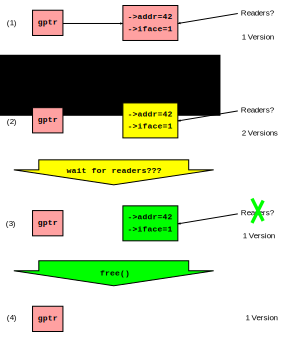
\includegraphics{defer/RCUListDeleteClassic}}
\caption{Deletion With Concurrent Readers}
\label{fig:defer:Deletion With Concurrent Readers}
\end{figure}

삽입은 물론 상당히 유용합니다만, 금방이든 더 나중이든, 데이터를 지워야 하기도
할 겁니다.
Figure~\ref{fig:defer:Deletion With Concurrent Readers}
에 보이듯, 첫번째 단계는 쉽습니다.
Section~\ref{sec:toolsoftrade:Shared-Variable Shenanigans}
에서의 교훈을 다시 상기해 보면, \co{smp_store_release()} 가 이 포인터를
\co{NULL} 로 만들기 위해 사용되어, 이 그림의 첫번째 열에서 두번째 열로
넘어갑니다.
이 시점에서, 기존부터 존재하던 읽기 쓰레드는 \co{->addr} 는 42 값을 그리고
\co{->iface} 는 1 값을 갖는 것으로 볼 수 있지만, 새로 시작된 읽기 쓰레드는
\co{NULL} 포인터를 볼 것으로, 즉 동시의 읽기 쓰레드들이 이 그림의 ``2
Versions'' 로 표시된 것처럼 현 상태에 대해 다른 의견을 가질 수 있습니다.

\iffalse

Insertion is of course quite useful, but sooner or later, it will also
be necessary to delete data.
As can be seen in
Figure~\ref{fig:defer:Deletion With Concurrent Readers},
the first step is easy.
Again taking the lessons from
Section~\ref{sec:toolsoftrade:Shared-Variable Shenanigans}
to heart, \co{smp_store_release()} is used to \co{NULL} the pointer,
thus moving from the first row to the second in the figure.
At this point, pre-existing readers see the old structure with
\co{->addr} of 42 and \co{->iface} of 1, but new readers will see
a \co{NULL} pointer, that is, concurrent readers can disagree on
the state, as indicated by the ``2 Versions'' in the figure.

\fi

\QuickQuizSeries{%
\QuickQuizB{
	Figure~\ref{fig:defer:Deletion With Concurrent Readers}
	는 \co{NULL} 포인터를 저장하는데 왜 \co{smp_store_release()} 를
	사용하나요?
	\co{NULL} 포인터 저장에 대해 순서지을 구조체 초기화가 없다는 점을
	감안하면 \co{WRITE_ONCE()} 만으로도 이 경우에는 괜찮지 않을까요?

	\iffalse

	Why does
	Figure~\ref{fig:defer:Deletion With Concurrent Readers}
	use \co{smp_store_release()} given that it is storing
	a \co{NULL} pointer?
	Wouldn't \co{WRITE_ONCE()} work just as well in this case,
	given that there is no structure initialization to order
	against the store of the \co{NULL} pointer?

	\fi

}\QuickQuizAnswerB{
	맞아요, 그럴 겁니다.

	\co{NULL} 포인터가 할당되고 있을 뿐, 순서지을 것이 존재하지 않으므로,
	\co{smp_store_release()} 를 사용할 필요는없습니다.
	대조적으로, \co{NULL} 이 아닌 포인터를 할당할 때에는 그 포인터로
	가리켜지는 구조체의 초기화가 이 포인터의 할당 전에 행해졌음을 분명히
	하기 위해 \co{smp_store_release()} 가 사용되어야 합니다.

	짧게 말해서, \co{WRITE_ONCE()} 는 동작할 것이고, 어떤 아키텍쳐에서는
	약간의 CPU 시간을 아낄 겁니다.
	하지만, 뒤에서 보게 되겠지만, 소프투에어 엔지니어링 관점의 걱정은
	\co{smp_store_release()} 와 상당히 유사한 \co{rcu_assign_pointer()}
	라는 특수한 기능의 사용을 장려할 겁니다.

	\iffalse

	Yes, it would.

	Because a \co{NULL} pointer is being assigned, there is nothing
	to order against, so there is no need for \co{smp_store_release()}.
	In contrast, when assigning a non-\co{NULL} pointer, it is
	necessary to use \co{smp_store_release()} in order to ensure
	that initialization of the pointed-to structure is carried
	out before assignment of the pointer.

	In short, \co{WRITE_ONCE()} would work, and would
	save a little bit of CPU time on some architectures.
	However, as we will see, software-engineering concerns
	will motivate use of a special \co{rcu_assign_pointer()}
	that is quite similar to \co{smp_store_release()}.

	\fi

}\QuickQuizEndB
%
\QuickQuizE{
	동시에 수행되는 읽기 쓰레드는
	Figure~\ref{fig:defer:Deletion With Concurrent Readers}
	에 그려진 수행 순서에 따르면 \co{gptr} 의 값에 대해 동의하지 않을 수
	있습니다.
	이건 뭔가 문제있지 않나요???

	\iffalse

	Readers running concurrently each other and with the procedure
	outlined in
	Figure~\ref{fig:defer:Deletion With Concurrent Readers}
	can disagree on the value of \co{gptr}.
	Isn't that just a wee bit problematic???

	\fi

}\QuickQuizAnswerE{
	꼭 그렇진 않습니다.

	Section~\ref{sec:cpu:Hardware Optimizations}
	와~\ref{sec:cpu:Hardware Free Lunch?}
	에서 힌트가 주어진 것처럼, 빛의 속도의 지연은 컴퓨터의 데이터는 그
	데이터가 실제로 모델링 하고자 의도된 바깥의 사실에 비교해서는 항상
	오래되어 있습니다.

	따라서 실제 세계의 알고리즘은 외부의 현실과 그 현실을 반영하는 컴퓨터
	내부 데이터의 비일관성을 감내해야만 합니다.
	이런 알고리즘들 여럿은 컴퓨터 내부 데이터에서의 비일관성도 어느정도는
	감내할 수 있습니다.
	Section~\ref{sec:datastruct:RCU-Protected Hash Table Discussion}
	이 이 점을 더 자세히 다룹니다.

	\iffalse

	Not necessarily.

	As hinted at in Sections~\ref{sec:cpu:Hardware Optimizations}
	and~\ref{sec:cpu:Hardware Free Lunch?},
	speed-of-light delays mean that a computer's data is always
	stale compared to whatever external reality that data is intended
	to model.

	Real-world algorithms therefore absolutely must tolerate
	inconsistancies between external reality and the in-computer
	data reflecting that reality.
	Many of those algorithms are also able to tolerate some degree
	of inconsistency within the in-computer data.
	Section~\ref{sec:datastruct:RCU-Protected Hash Table Discussion}
	discusses this point in more detail.

	\fi

	이런 비일관적이고 오래된 데이터를 감내해야 하는 필요성은 RCU 에만
	국한되지 않는다는 점을 알아두시기 바랍니다.
	이는 레퍼런스 카운팅, 해저드 포인터, 시퀀스 락, 그리고 심지어 일부 락킹
	사용 예에도 적용됩니다.
	예를 들어, 여러분이 락을 잡은 채 어떤 값을 계산하지만 그 값을 해당 락을
	해제한 후 사용한다면, 여러분은 오래된 데이터를 사용하고 있을 수
	있습니다.
	어쨌건, 그 값이 기반하고 있는 데이터는 그 락이 해제되는 순간 어떻게든
	변할 수도 있습니다.

	그러니, 그렇습니다, RCU 읽기 쓰레드는 오래되고 비일관적인 데이터를 볼
	수 있습니다, 하지만 아니요, 이게 문제여야만 할 이유는 없어요.
	그리고 필요하다면 그런 오래되고 비일관적인 데이터 문제를 막을 수 있는
	RCU 사용 패턴도 있습니다~\cite{Arcangeli03}.

	\iffalse

	Please note that this need to tolerate inconsistent and stale
	data is not limited to RCU\@.
	It also applies to reference counting, hazard pointers, sequence
	locks, and even to some locking use cases.
	For example, if you compute some quantity while holding a lock,
	but use that quantity after releasing that lock,
	you might well be using stale data.
	After all, the data that quantity is based on might change
	arbitrarily as soon as the lock is released.

	So yes, RCU readers can see stale and inconsistent data, but no,
	this is not necessarily problematic.
	And, when needed, there are RCU usage patterns that avoid both
	staleness and inconsistency~\cite{Arcangeli03}.

	\fi

}\QuickQuizEndE
}

우린 열~3 에서 볼 수 있듯 모든 기존부터 존재한 읽기 쓰레드들이 완료하길
기다리는 것만으로 단일 버전으로 돌아올 수 있습니다.
이 지점에서, 모든 기존부터 존재하던 읽기 쓰레드는 종료되었고, 뒤따르는 읽기
쓰레드는 어느 것도 기존 데이터 아이템으로의 경로를 갖지 못하므로, 그걸 참조하는
어떤 읽기 쓰레드도 존재할 수 없습니다.
따라서 그 아이템은 열~4 에서 보여지듯 안전히 메모리 해제될 수 있습니다.

따라서, 기존부터 존재한 읽기 쓰레드들이 완료되길 기다릴 방법이 존재한다면
읽기 쓰레드들이 싱글 쓰레드 수행 시에나 적합할 것과 동일한 기계
인스트럭션들만을 수행하면서도 연결된 데이터 구조에 데이터를 추가할 수도 삭제할
수도 있습니다.
그러니 앞서 했던 것들이 너무 멀리 간 것만은 아닐수도 있습니다!

하지만 어떻게 기존부터 존재한 읽기 쓰레드들이 실제로 완료되었다고 이야기 할 수
있을까요?
이 질문이 다음 섹션의 주제입니다.

\iffalse

We get back to a single version simply by waiting for all the
pre-existing readers to complete, as shown in row~3.
At that point, all the pre-existing readers are done, and no later
reader has a path to the old data item, so there can no longer be
any readers referencing it.
It may therefore be safely freed, as shown on row~4.

Thus, given a way to wait for pre-existing readers to complete,
it is possible to both add data to and remove data from a linked
data structure, despite the readers executing the same sequence
of machine instructions that would be appropriate for single-threaded
execution.
So perhaps going all the way was not too far after all!

But how can we tell when all of the pre-existing readers have in
fact completed?
This question is the topic of the next section.

\fi

\subsubsection{Waiting for Readers}
\label{sec:defer:Waiting for Readers}

It is tempting to base reader waiting on reference counting, but
Figure~\ref{fig:count:Atomic Increment Scalability on x86}
in
Chapter~\ref{chp:Counting}
shows that concurrent reference counting results in extreme overhead,
as we already saw in
Section~\ref{sec:defer:Reference Counting}.
Hazard pointers profoundly reduce this overhead, but, as we saw in
Section~\ref{sec:defer:Hazard Pointers}, not to zero.
Nevertheless, many RCU implementations make very careful cache-local
use of counters.

A second approach observes that memory synchronization is expensive,
and therefore uses registers instead, namely each CPU's or thread's
program counter (PC), thus imposing no overhead on readers, at least
in the absence of concurrent updates.
The updater polls each relevant PC, and if that PC is not within read-side
code, then the corresponding CPU or thread is within a quiescent state,
in turn signaling the completion of any reader that might have access
to the newly removed data element.
Once all CPU's or thread's PCs have been observed to be outside of any
reader, the grace period has completed.
Please note that this approach poses some serious challenges, including
memory ordering, functions that are \emph{sometimes} invoked from readers,
and ever-exciting code-motion optimizations.
Nevertheless, this approach is said to be used in
production~\cite{MikeAsh2015Apple}.

A third approach is to simply wait for a fixed period of time that is
long enough to comfortably exceed the lifetime of any reasonable
reader~\cite{Jacobson93,AjuJohn95}.
This can work quite well in hard real-time systems~\cite{YuxinRen2018RTRCU},
but in less exotic
settings, Murphy says that it is critically important to be prepared
even for unreasonably long-lived readers.
To see this, consider the consequences of failing do so:
A data item will be freed while the unreasonable reader is still
referencing it, and that item might well be immediately reallocated,
possibly even as a data item of some other type.
The unreasonable reader and the unwitting reallocator would then
be attempting to use the same memory for two very different purposes.
The ensuing mess will at best be exceedingly difficult to debug.

A fourth approach is to wait forever, secure in the knowledge that
doing so will accommodate even the most unreasonable reader.
This approach is also called ``leaking memory'', and has a bad reputation
due to the fact that memory leaks often require untimely and
inconvenient reboots.
Nevertheless, this is a viable strategy when the update rate and the
uptime are both sharply bounded.
For example, this approach could work well in a high-availability
cluster where systems were periodically crashed in order to ensure
that cluster really remained highly available.\footnote{
	The program that forces the periodic crashing is sometimes
	known as a ``chaos monkey'':
	\url{https://netflix.github.io/chaosmonkey/}.
	However, it might also be a mistake to neglect chaos caused
	by systems running for too long.}
Leaking the memory is also a viable strategy in environments having
garbage collectors, in which case the garbage collector can be thought
of as plugging the leak~\cite{Kung80}.
However, if your environment lacks a garbage collector, read on!

A fifth approach avoids the period crashes in favor of periodically
``stopping the world'', as exemplified by the traditional stop-the-world
garbage collector.
This approach was also heavily used during the decades before
ubiquitous connectivity, when it was common practice to power systems
off at the end of each working day.
However, in today's always-connected always-on world, stopping the world
can gravely degrade response times, which has been one motivation for the
development of concurrent garbage collectors~\cite{DavidFBacon2003RTGC}.
Furthermore, although we need all pre-existing readers to complete, we do
not need them all to complete at the same time.

This observation leads to the sixth approach, which is stopping
one CPU or thread at a time.
This approach has the advantage of not degrading reader response times
at all, let alone gravely.
Furthermore, numerous applications already have states (termed
\emph{quiescent states}) that can be
reached only after all pre-existing readers are done.
In transaction-processing systems, the time between a pair of
successive transactions might be a quiescent state.
In reactive systems, the state between a pair of successive events
might be a quiescent state.
Within non-preemptive operating-systems kernels, a context switch can be
a quiescent state~\cite{McKenney98}.
Either way, once all CPUs and/or threads have passed through a quiescent
state, the system is said to have completed a \emph{grace period},
at which point all readers in existence at the start of that grace period
are guaranteed to have completed.
As a result, it is also guaranteed to be safe to free any removed data
items that were removed prior to the start of that grace period.\footnote{
	It is possible to do much more with RCU than simply defer
	reclamation of memory, but deferred reclamation is RCU's most
	common use case, and is therefore an excellent place to start.}

Within a non-preemptive operating-system kernel, for context switch to be
a valid quiescent state, readers must be prohibited from blocking while
referencing a given instance data structure obtained via the \co{gptr}
pointer shown in
Figures~\ref{fig:defer:Insertion With Concurrent Readers}
and~\ref{fig:defer:Deletion With Concurrent Readers}.
This no-blocking constraint is consistent with similar constraints
on pure spinlocks, where a CPU is forbidden from blocking while
holding a spinlock.
Without this constraint, all CPUs might be consumed by threads
spinning attempting to acquire a spinlock held by a blocked thread.
The spinning threads will not relinquish their CPUs until they acquire
the lock, but the thread holding the lock cannot possibly release it
until one of the spinning threads relinquishes a CPU\@.
This is a classic deadlock situation, and this deadlock is avoided
by forbidding blocking while holding a spinlock.

Again, this same constraint is imposed on reader threads dereferencing
\co{gptr}: such threads are not allowed to block until after
they are done using the pointed-to data item.
Returning to the second row of
Figure~\ref{fig:defer:Deletion With Concurrent Readers},
where the updater has just completed executing the \co{smp_store_release()},
imagine that CPU~0 executes a context switch.
Because readers are not permitted to block while traversing the linked
list, we are guaranteed that all prior readers that might have been running on
CPU~0 will have completed.
Extending this line of reasoning to the other CPUs, once each CPU has
been observed executing a context switch, we are guaranteed that all
prior readers have completed, and that there are no longer any reader
threads referencing the newly removed data element.
The updater can then safely free that data element, resulting in the
state shown at the bottom of
Figure~\ref{fig:defer:Deletion With Concurrent Readers}.

\begin{figure}[tb]
\centering
\resizebox{3in}{!}{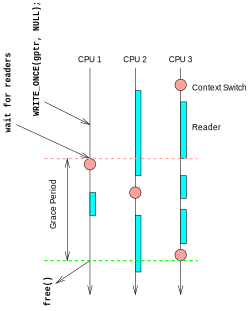
\includegraphics{defer/QSBRGracePeriod}}
\caption{QSBR: Waiting for Pre-Existing Readers}
\label{fig:defer:QSBR: Waiting for Pre-Existing Readers}
\end{figure}

This approach is termed \emph{quiescent state based reclamation}
(QSBR)~\cite{ThomasEHart2006a}.
A QSBR schematic is shown in
Figure~\ref{fig:defer:QSBR: Waiting for Pre-Existing Readers},
with time advancing from the top of the figure to the bottom.
CPU~1 does the \co{WRITE_ONCE()} that removes the current data
item (presumably having previously read the pointer value and
availed itself of appropriate synchronization), then waits
for readers.
This wait operation results in an immediate context switch, which is a
quiescent state (denoted by the pink circle), which in turn means that
all prior reads on CPU~1 have completed.
Next, CPU~2 does a context switch, so that all readers on CPUs~1 and~2
are now known to have completed.
Finally, CPU~3 does a context switch.
At this point, all readers throughout the entire system are known to
have completed, so the grace period ends, permitting CPU~1 to free
the old data item.

\QuickQuiz{
	In Figure~\ref{fig:defer:QSBR: Waiting for Pre-Existing Readers},
	the last of CPU~3's readers that could possibly have
	access to the old data item ended before the grace period
	even started!
	So why would anyone bother waiting until CPU~3's later context
	switch???
}\QuickQuizAnswer{
	Because that waiting is exactly what enables readers to use
	the same sequence of instructions that is appropriate for
	single-theaded situations.
	In other words, this additional ``redundant'' waiting enables
	excellent read-side performance, scalability, and real-time
	response.
}\QuickQuizEnd

\subsubsection{Toy Implementation}
\label{sec:defer:Toy Implementation}

Although production-quality QSBR implementations can be quite complex,
a toy non-preemptive Linux-kernel implementation is exceedingly simple:

\begin{VerbatimN}[samepage=true]
void synchronize_rcu(void)
{
	int cpu;

	for_each_online_cpu(cpu)
		sched_setaffinity(current->pid, cpumask_of(cpu));
}
\end{VerbatimN}

The \co{for_each_online_cpu()} primitive iterates over all CPUs, and
the \co{sched_setaffinity()} function causes the current thread to
execute on the specified CPU, which forces the destination CPU to execute
a context switch.
Therefore, once the \co{for_each_online_cpu()} has completed, each CPU
has executed a context switch, which in turn guarantees that
all pre-existing reader threads have completed.

\begin{listing}[tbp]
\begin{fcvlabel}[ln:defer:Insertion and Deletion With Concurrent Readers]
\begin{VerbatimL}[commandchars=\\\[\]]
struct route *gptr;

int access_route(int (*f)(struct route *rp))
{
	int ret = -1;
	struct route *rp;

	rcu_read_lock();
	rp = rcu_dereference(gptr);
	if (rp)
		ret = f(rp);		\lnlbl[access_rp]
	rcu_read_unlock();
	return ret;
}

struct route *ins_route(struct route *rp)
{
	struct route *old_rp;

	spin_lock(&route_lock);
	old_rp = gptr;
	rcu_assign_pointer(gptr, rp);
	spin_unlock(&route_lock);
	return old_rp;
}

int del_route(void)
{
	struct route *old_rp;

	spin_lock(&route_lock);
	old_rp = gptr;
	RCU_INIT_POINTER(gptr, NULL);
	spin_unlock(&route_lock);
	synchronize_rcu();
	free(old_rp);
	return !!old_rp;
}
\end{VerbatimL}
\end{fcvlabel}
\caption{Insertion and Deletion With Concurrent Readers}
\label{lst:defer:Insertion and Deletion With Concurrent Readers}
\end{listing}

Please note that this approach is \emph{not} production quality.
Correct handling of a number of corner cases and the need for a number
of powerful optimizations mean that production-quality implementations
are quite complex.
In addition, RCU implementations for preemptible environments
require that readers actually do something, which in non-real-time
Linux-kernel environments can be as simple as defining
\co{rcu_read_lock()} and \co{rcu_read_unlock()} as \co{preempt_disable()}
and \co{preempt_enable()}, respectively.\footnote{
	Some toy RCU implementations that handle preempted
	read-side critical sections are shown in
	Appendix~\ref{chp:app:``Toy'' RCU Implementations}.}
However, this simple non-preemptible approach is conceptually complete,
and demonstrates that it really is possible to provide read-side
synchronization at zero cost, even in the face of concurrent updates.
In fact,
Listing~\ref{lst:defer:Insertion and Deletion With Concurrent Readers}
shows how reading (\co{access_route()}),
Figure~\ref{fig:defer:Insertion With Concurrent Readers}'s
insertion (\co{ins_route()}) and
Figure~\ref{fig:defer:Deletion With Concurrent Readers}'s
deletion (\co{del_route()}) can
be implemented.
(A slightly more capable routing table is shown in
Section~\ref{sec:defer:RCU for Pre-BSD Routing}.)

\QuickQuizSeries{%
\QuickQuizB{
	What is the point of \co{rcu_read_lock()} and \co{rcu_read_unlock()} in
	Listing~\ref{lst:defer:Insertion and Deletion With Concurrent Readers}?
	Why not just let the quiescent states speak for themselves?
}\QuickQuizAnswerB{
	Recall that readers are not permitted to pass through a quiescent
	state.
	For example, within the Linux kernel, RCU readers are not permitted
	to execute a context switch.
	Use of \co{rcu_read_lock()} and \co{rcu_read_unlock()} enables
	debug checks for improperly placed quiescent states, making it
	easy to find bugs that would otherwise be difficult to find,
	intermittent, and quite destructive.
}\QuickQuizEndB
%
\QuickQuizE{
	What is the point of \co{rcu_dereference()}, \co{rcu_assign_pointer()}
	and \co{RCU_INIT_POINTER()} in
	Listing~\ref{lst:defer:Insertion and Deletion With Concurrent Readers}?
	Why not just use \co{READ_ONCE()}, \co{smp_store_release()}, and
	\co{WRITE_ONCE()}, respectively?
}\QuickQuizAnswerE{
	The RCU-specific APIs do have similar semantics to the suggested
	replacements, but also enable static-analysis debugging checks
	that complain if an RCU-specific API is invoked on a non-RCU
	pointer and vice versa.
}\QuickQuizEndE
}

Referring back to
Listing~\ref{lst:defer:Insertion and Deletion With Concurrent Readers},
note that \co{route_lock} is used to synchronize between concurrent updaters
invoking \co{ins_route()} and \co{del_route()}.
However, this lock is not acquired by readers invoking \co{access_route()}:
Readers are instead protected by the QSBR techniques described in this section.

Note that \co{ins_route()} simply returns the old value of \co{gptr}, which
Figure~\ref{fig:defer:Insertion With Concurrent Readers} assumed would
always be \co{NULL}.
This means that it is the caller's responsibility to figure out what to
do with a non-\co{NULL} value, a task complicated by the fact that
readers might still be referencing it for an indeterminate period of time.
Callers might use one of the following approaches:

\begin{enumerate}
\item	Use \co{synchronize_rcu()} to safely free the pointed-to structure.
	Although this approach is correct from an RCU perspective, it
	arguably has software-engineering leaky-API problems.
\item	Trip an assertion if the returned pointer is non-\co{NULL}.
\item	Pass the returned pointer to a later invocation of
	\co{ins_route()} to restore the earlier value.
\end{enumerate}

In contrast, \co{del_route()} uses \co{synchronize_rcu()} and
\co{free()} to safely free the newly deleted data item.

\QuickQuiz{
	But what if the old structure needs to be freed, but the caller
	of \co{ins_route()} cannot block, perhaps due to performance
	considerations or perhaps because the caller is executing within
	an RCU read-side critical section?
}\QuickQuizAnswer{
	A \co{call_rcu()} function, which is described in
	Section~\ref{sec:defer:Wait For Pre-Existing RCU Readers},
	permits asynchronous grace-period waits.
}\QuickQuizEnd

This example shows one general approach to reading and updating
RCU-protected data structures, however, there is quite a variety
of use cases, several of which are covered in
Section~\ref{sec:defer:RCU Usage}.

In summary, it is in fact possible to create concurrent linked data
structures that can be traversed by readers executing the same sequence
of machine instructions that would be executed by single-threaded readers.
The next section summarizes RCU's high-level properties.

\subsubsection{RCU Properties}
\label{sec:defer:RCU Properties}

A key RCU property is that reads need not wait for updates.
This property enables RCU implementations to provide low-cost or even
no-cost readers, resulting in low overhead and excellent scalability.
This property also allows RCU readers and updaters to make useful
concurrent forward progress.
In contrast, conventional synchronization primitives must enforce strict
mutual exclusion using expensive instructions, thus increasing overhead
and degrading scalability, but also typically prohibiting readers and
updaters from making useful concurrent forward progress.

\QuickQuiz{
	Doesn't Section~\ref{sec:defer:Sequence Locks}'s seqlock
	also permit readers and updaters to make useful concurrent
	forward progress?
}\QuickQuizAnswer{
	Yes and no.
	Although seqlock readers can run concurrently with
	seqlock writers, whenever this happens, the \co{read_seqretry()}
	primitive will force the reader to retry.
	This means that any work done by a seqlock reader running concurrently
	with a seqlock updater will be discarded and the redone upon retry.
	So seqlock readers can \emph{run} concurrently with updaters,
	but they cannot actually get any work done in this case.

	In contrast, RCU readers can perform useful work even in presence
	of concurrent RCU updaters.

	However, both reference counters
	(Section~\ref{sec:defer:Reference Counting})
	and hazard pointers
	(Section~\ref{sec:defer:Hazard Pointers})
	really do permit useful concurrent forward progress for both
	updaters and readers, just at somewhat greater cost.
	Please see
	Section~\ref{sec:defer:Which to Choose?}
	for a comparison of these different solutions to the
	deferred-reclamation problem.
}\QuickQuizEnd

RCU delimits readers with \co{rcu_read_lock()} and \co{rcu_read_unlock()},
and ensures that each reader has a coherent view of each object
(see \cref{fig:defer:Deletion With Concurrent Readers}) by
maintaining multiple versions of objects and using update-side primitives
such as \co{synchronize_rcu()} to ensure that objects are not
freed until after the completion of all readers that might be using them.
RCU uses \co{rcu_assign_pointer()} and \co{rcu_dereference()} to provide
efficient and scalable mechanisms for publishing and reading new versions
of an object, respectively.
These mechanisms distribute the work among read and
update paths in such a way as to make read paths extremely fast, using
replication and weakening optimizations in a manner similar to
hazard pointers, but without the need for read-side retries.
In some cases, including \co{CONFIG_PREEMPT=n} Linux kernels,
RCU's read-side primitives have zero overhead.

But are these properties actually useful in practice?
This question is taken up by the next section.

\subsubsection{Practical Applicability}
\label{sec:defer:Practical Applicability}

\begin{figure}[tb]
\centering
\resizebox{3in}{!}{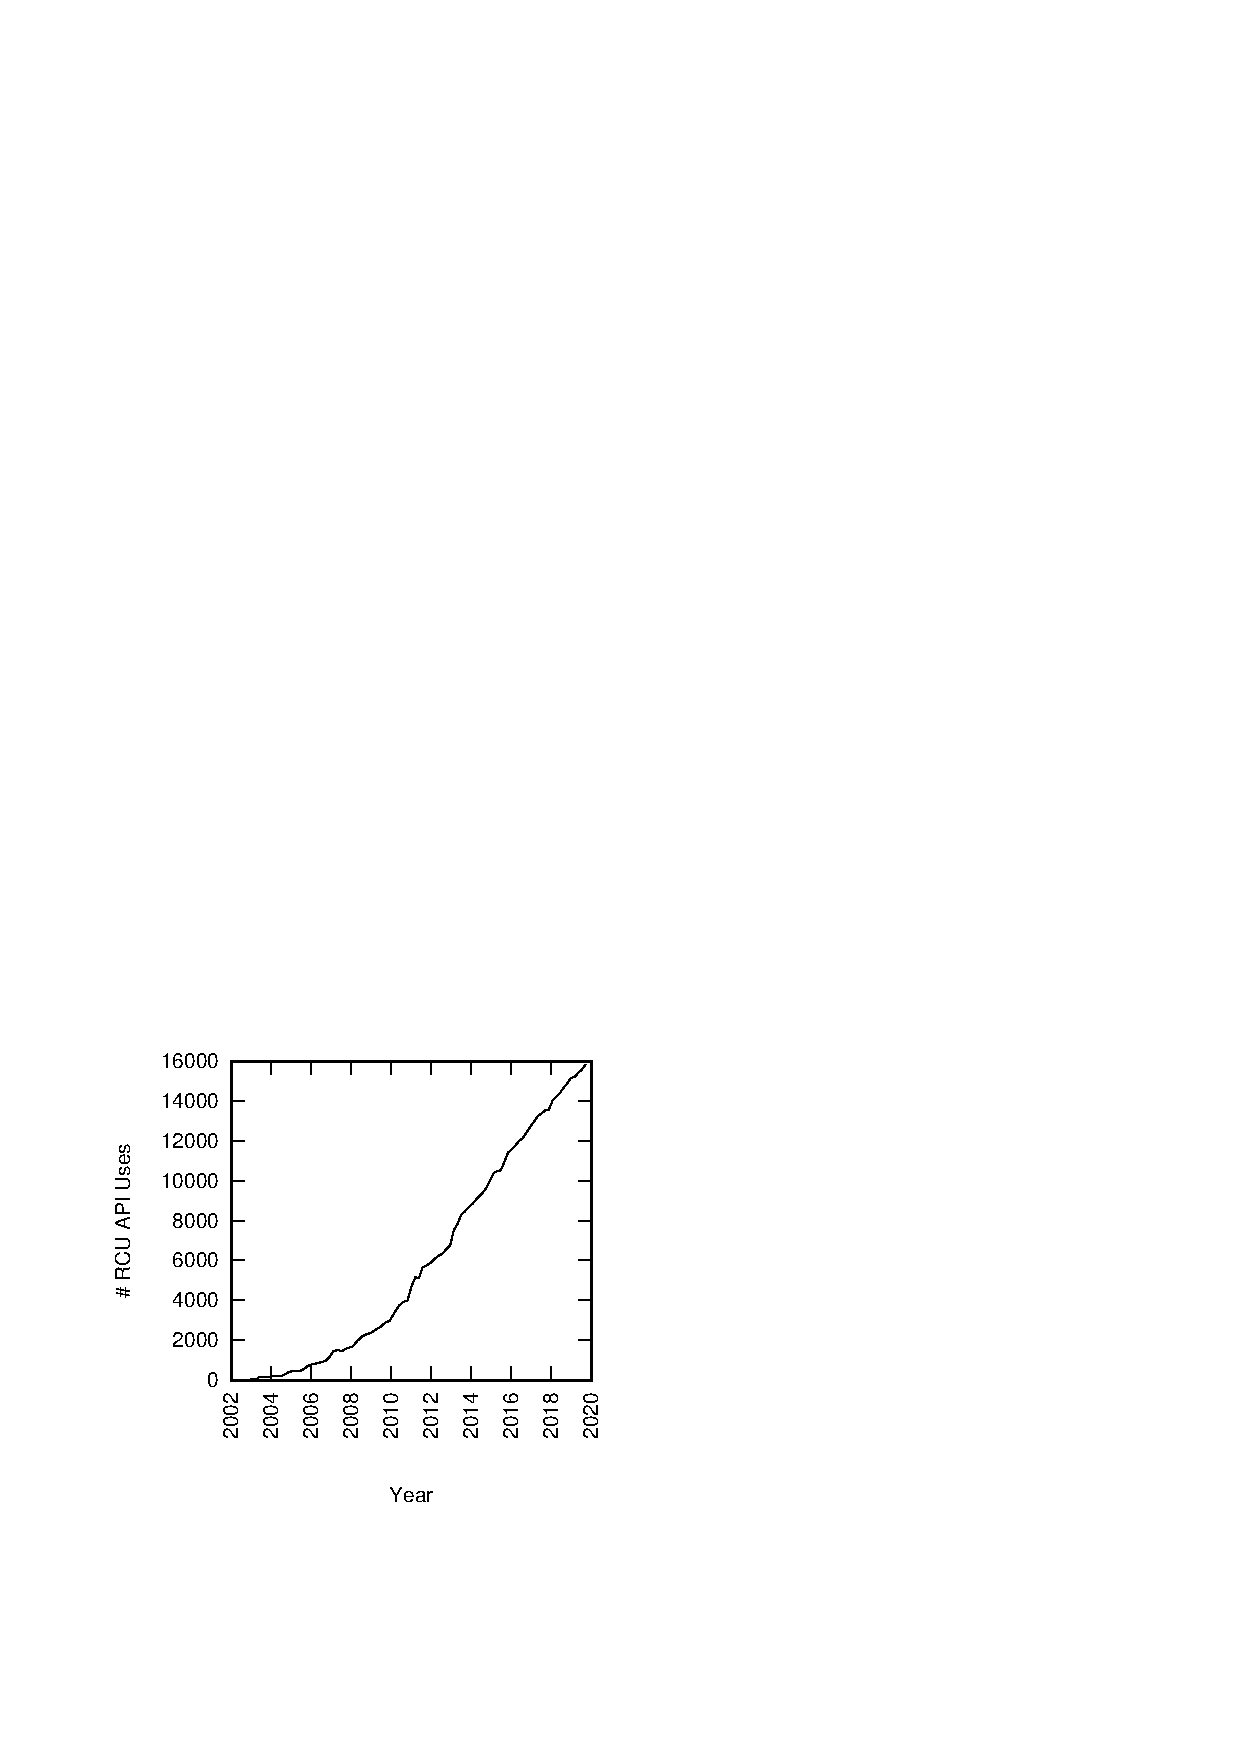
\includegraphics{defer/linux-RCU}}
\caption{RCU Usage in the Linux Kernel}
\label{fig:defer:RCU Usage in the Linux Kernel}
\end{figure}

RCU has been used in the Linux kernel since
October 2002~\cite{Torvalds2.5.43}.
Use of the RCU API has increased substantially since that time,
as can be seen in
Figure~\ref{fig:defer:RCU Usage in the Linux Kernel}.
In fact, code very similar to that in
Listing~\ref{lst:defer:Insertion and Deletion With Concurrent Readers}
is used in the Linux kernel.
RCU has enjoyed heavy use both prior to and since its acceptance
in the Linux kernel, as discussed in
\cref{sec:defer:RCU Related Work}.

It is therefore safe to say that RCU enjoys wide practical applicability.

The minimal example discussed in this section is a good introduction to RCU\@.
However, effective use of RCU often requires that you think differently
about your problem.
It is therefore useful to examine RCU's fundamentals, a task taken up
by the following section.
